%! TEX root = **/000-main.tex
% vim: spell spelllang=en:

% Using the figure from the slides, instantiate it (i.e., add on top) the tools
% you used for each element from the architecture.

\section{Data analysis backbone}

\begin{figure}[H]
    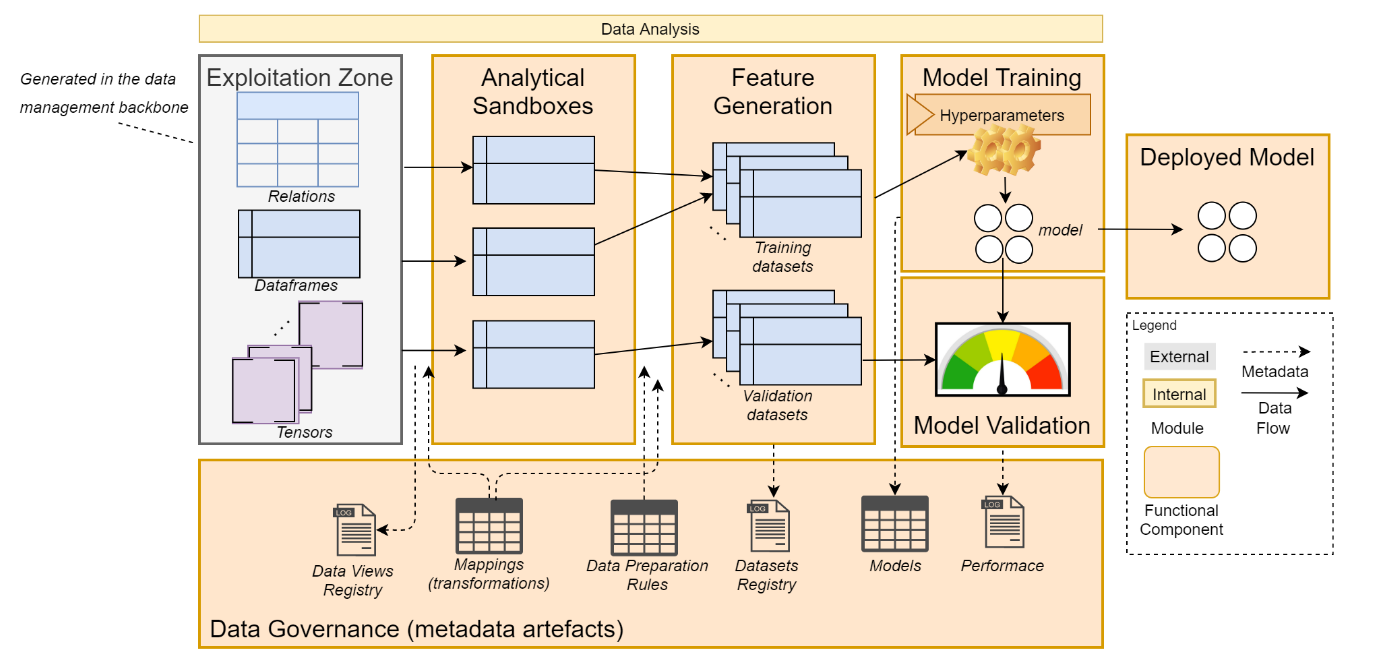
\includegraphics[width=\linewidth]{data-analysis-backbone}
\end{figure}

In the exploitation zone, we integrate the data into a single source table. To do so, we first join all the tables related to deaths and all the tables related to demographic information. After that, we join these two by year and country name.

We perform some pivots to obtain a more suitable dataframe, and we also generate some additional features. Finally, the train and test datasets are created and stored in the dataset folder.

We create a pipeline in which we first do a simple imputation of missing values, and then we use a grid based cross-validation approach to estimate the best parameters of a random forest regression. We persist the trained model in the model folder, versioned by timestamp.